\section{AI-Assisted Documentation Generation}

This chapter describes how LivingDocs uses Artificial Intelligence to automatically generate technical documentation from source code while maintaining traceability and human verification before publication.

The design combines Static Code Analysis, Abstract Syntax Tree (AST), Retrieval-Augmented Generation (RAG), and Large Language Models (LLMs) to produce documentation that remains synchronized with repository changes.

%================================================

\section{Architecture Overview}

The AI documentation module follows the workflow below.

\begin{enumerate}
    \item Repository synchronization.
    \item Source code parsing.
    \item AST extraction.
    \item Semantic context construction.
    \item AI documentation generation.
    \item Human review.
    \item Publication.
\end{enumerate}

%================================================

\section{Documentation Generation Workflow}

The Activity Diagram illustrates the complete AI documentation generation process.

\begin{figure}[H]
    \centering
    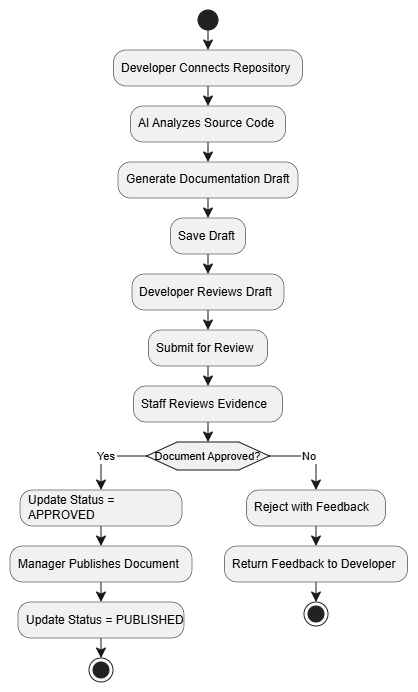
\includegraphics[width=\textwidth]{images/Activity_Diagram.png}
    \caption{AI Documentation Generation Activity Diagram}
    \label{fig:activity-ai}
\end{figure}

%================================================

\section{Component Responsibilities}

\begin{longtable}{|p{4cm}|p{8cm}|}
\hline
\textbf{Component} & \textbf{Responsibility}\\
\hline
GitHub Integration & Receives repository events through Webhooks.\\
\hline
Source Parser & Reads project files and extracts syntax information.\\
\hline
AST Engine & Builds Abstract Syntax Trees for supported languages.\\
\hline
Context Builder & Creates semantic context for AI processing.\\
\hline
RAG Pipeline & Retrieves relevant documentation before generation.\\
\hline
LLM Generator & Produces technical documentation drafts.\\
\hline
Review Engine & Sends generated drafts to human reviewers.\\
\hline
Version Manager & Stores document versions and audit history.\\
\hline
\end{longtable}

%================================================

\section{AST-Based Analysis}

Instead of relying only on raw source code, LivingDocs first constructs an Abstract Syntax Tree (AST).

The AST enables the system to identify:

\begin{itemize}
    \item Classes
    \item Functions
    \item Parameters
    \item Return types
    \item Dependencies
    \item Structural relationships
\end{itemize}

This structured representation improves documentation accuracy compared with plain-text generation.

%================================================

\section{Retrieval-Augmented Generation}

The RAG pipeline enriches prompts with existing documentation before AI generation.

The process consists of:

\begin{enumerate}
    \item Retrieve related documentation.
    \item Combine retrieved context with AST information.
    \item Generate updated documentation.
    \item Return grounded output.
\end{enumerate}

Grounding evidence is displayed so reviewers can verify every generated section.

%================================================

\section{Output Verification}

Every generated document includes:

\begin{itemize}
    \item Source code references.
    \item Version information.
    \item Generation timestamp.
    \item Review status.
\end{itemize}

This design ensures that AI-generated content remains transparent and verifiable before publication.